\section*{Условие}

\begin{figure}[H]
    \begin{center}
        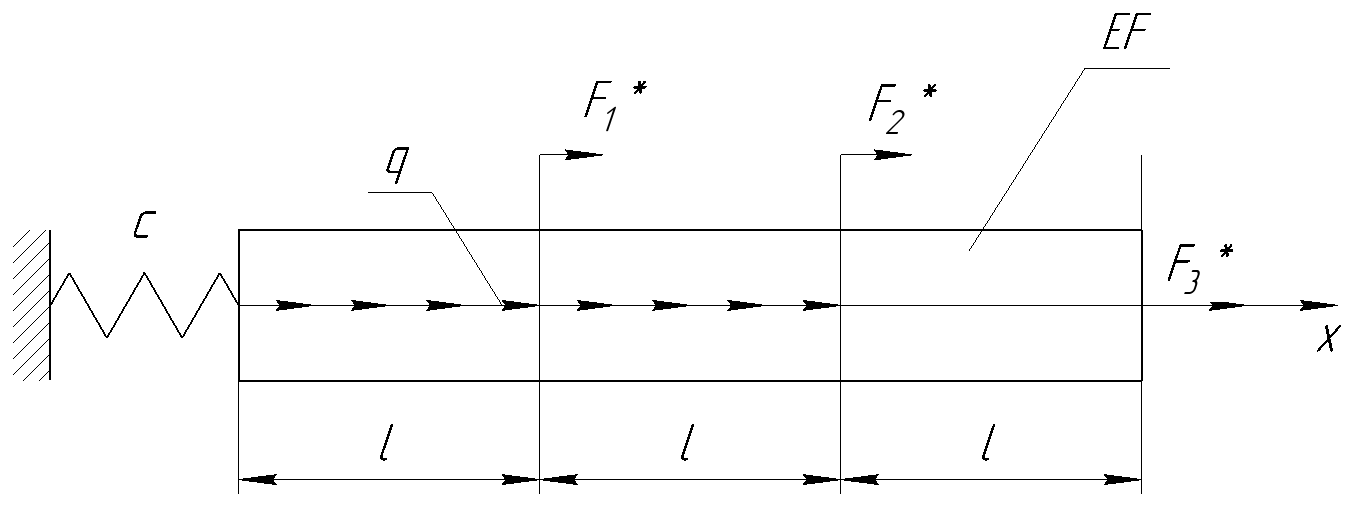
\includegraphics[width = 0.7\linewidth]{1.png}
        \caption*{Расчетная схема}
        \label{pic0.1}
    \end{center}
\end{figure}

Для данной расчетной схемы необходимо:

\textbf{Часть 1.}
\begin{enumerate}
    \item Сформулировать краевую задачу.
    \item Построить точное решение краевой задачи.
    \item Преобразовать краевую задачу в вариационный принцип
    \item Получить решение энергетическим методом на линейной аппроксимации поля перемещений
    \item Дать оценку погрешности по энергии между точным и приближенным решением
    \\ \textbf{Часть 2.}
    \item Записать разрешающую систему уравнений Метода Конечных Элементов (МКЭ), провести ее анализ и получить <<вручную>> решение для перемещений и напряжений
    \item Выполнить расчет заданной конструкции с использованием пакета MSC Patran\_Nastran
    \item Провести сравнительный анализ результатов, полученных методами, использованными в работе.
    \item Подготовить отчет по результатам проведенных исследований
\end{enumerate}

Согласно варианту №13 имеем следующие исходные данные:
\begin{equation}
    \label{eq0.1}
    \begin{cases}
        \displaystyle \frac{cl}{EF} = 7
        \\[10pt]
        \displaystyle \frac{ql}{EF} = 1
        \\[10pt]
        \displaystyle \frac{F_1^*}{EF} = 0
        \\[10pt]
        \displaystyle \frac{F_2^*}{EF} = 0.5
        \\[10pt]
        \displaystyle \frac{F_3^*}{EF} = 0.2
    \end{cases}
\end{equation}

При выполнении численных расчетов принять следующие значения параметров:
\begin{itemize}
    \item Площадь поперечного сечения $F = a \cdot b = 0.1 \t{м} \cdot 0.15 \t{м} = 0.015 \t{м}^2$
    \item Длина участка $l = 0.5 \t{м}$
    \item Для варианта №13 материал: Дюраль ($E = 7.31 \cdot 10^{10}\; \t{Па}; \nu = 0.33$)
\end{itemize}